\input sys/inputs.tex

\begin{document}

\bigheading{Skiing}

% \info{task_name}{infile}{outfile}{points}{timelimit}{memlimit}
% leave this values, if you are not interested
\info{skiing}{stdin}{stdout}{100}{1000 ms}{1 GB}

After an unsuccessful attempt to qualify for IOI, Kleofáš decided to become
a slalom skiing champion. Tomorrow is a very important day in Kleofáš's life:
he will compete in his very first skiing contest!

During the contest, Kleofáš will have to get from a starting point to a finishing point,
while passing through $n$ gates. In order to be as fast as possible, Kleofáš wants
to use the shortest possible trajectory.

\heading{Task}

A skiing course can be described as a starting point $S$, a finishing point $F$ and $n$ 
gates. Each gate is a line segment parallel to the $x$ axis (i. e. horizontal). No two
gates are at the same $y$ coordinate (altitude). The starting point is above each gate
i. e. its $y$ coordinate is higher than $y$ coordinate of any gate. The finishing point
is below each gate.

Find the shortest polygonal chain starting at point $S$, finishing at point $F$ and intersecting
all gates, in order \textbf{from top to bottom}. We say that a polygonal chain intersects a line
segment if they have at least one common point (this point \textbf{can} be an endpoint of the line segment).

\heading{Input}

First line of the input contains one integer $n$ ($0 \leq n \leq 10^6$) -- number of gates.
Second line contains four integers $x_S, y_S, x_F, y_F$: coordinates of points $S = (x_S, y_S)$
and $F = (x_F, y_F)$ respectively.

$n$ lines follow, $i$-th of them contains three integers ${x_1}_i, {x_2}_i, {y}_i$, meaning that
$i$-th gate is a segment from $({x_1}_i, y_i)$ to $({x_2}_i, y_i)$. For each $i$, 
${x_1}_i < {x_2}_i$ holds.

All coordinates are between $-10^9$ and $10^9$, inclusive. Gates are ordered from top to bottom,
i. e. $y_S > y_1 > y_2 > \dots > y_n > y_F$.

\heading{Output}

It can be proven that there always exists a unique shortest polygonal chain and all its vertices have integer coordinates. Output this chain without any redundant vertices (i. e. only output vertices
where the chain changes its direction).

\begin{center}
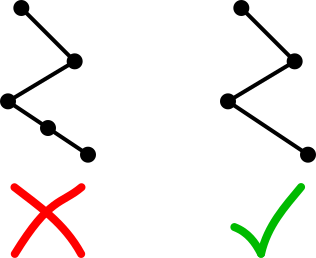
\includegraphics[width=5cm]{img/skiing1}
\end{center}

On the first line of the output print a single integer $k$ -- number of vertices in the optimal chain. Then print $k$ more lines, $i$-th of them containing two space-separated integers $x_i, y_i$ -- coordinates of the $i$-th vertex of the chain. Vertices must be named from the start of the chain to the
end, thus
$x_1 = x_S, y_1 = y_S, x_k = x_F, y_k = y_F$ and $y_1 > y_2 > \dots > y_k$ must hold.

\heading{Samples}


\sampleIN
4
5 10 6 0
0 4 7
7 10 6
5 8 4
2 5 1
\sampleOUT
5
5 10
4 7
7 6
5 1
6 0
\sampleCOMMENT
The situation looks like this:
\sampleEND
\center{
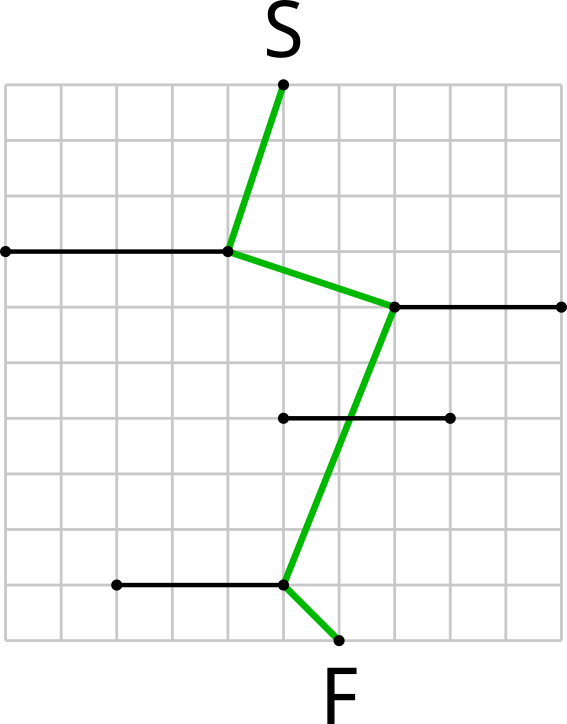
\includegraphics[width=6cm]{img/skiing2}
}

\end{document}
